%\documentclass[preprint,linenumbers,superscriptaddress]{revtex4-2}
\documentclass[onecolumn,superscriptaddress]{revtex4-2}

\usepackage{graphicx}% Include figure files
\usepackage{dcolumn}% Align table columns on decimal point
\usepackage{bm}% bold math
\usepackage{mathtools}
\usepackage{amsmath, amssymb}
\usepackage{bbold}
\usepackage{textcomp}
\usepackage{tabulary,graphicx,amsmath,amsfonts,amssymb}
\usepackage{float}
% \usepackage[utf8x]{inputenc}
% \usepackage[T1]{fontenc}
\usepackage{titlesec}
\usepackage[breaklinks = true]{hyperref}


% \def\GITURL{https://}

\DeclarePairedDelimiter\bra{\langle}{\rvert}
\DeclarePairedDelimiter\ket{\lvert}{\rangle}
\DeclarePairedDelimiterX\braket[2]{\langle}{\rangle}{#1 \delimsize\vert #2}
% \documentclass[onecolumn,superscriptaddress]{revtex4-2}

% \usepackage{textcomp}
% \usepackage{tabulary,graphicx,amsmath,amsfonts,amssymb}
% \usepackage{float}
% \usepackage[utf8x]{inputenc}
% \usepackage[T1]{fontenc}
% \usepackage{titlesec}
% \usepackage[breaklinks = true]{hyperref}

\renewcommand{\baselinestretch}{1.5}
\newcommand\new[1]{\textcolor{red}{#1}}
\hypersetup{
    colorlinks=true,
    linkcolor=blue,
    filecolor=magenta,      
    urlcolor=blue,
    citecolor=red
}
\urlstyle{same}


\graphicspath{ {./images_si/} }

\usepackage{url,multirow,morefloats,floatflt,cancel,tfrupee}
\makeatletter


\AtBeginDocument{\@ifpackageloaded{textcomp}{}{\usepackage{textcomp}}}
\makeatother
\usepackage{colortbl}
\usepackage{xcolor}
\usepackage{pifont}
\usepackage[nointegrals]{wasysym}
\urlstyle{rm}
\makeatletter

\def\bibsection{\section*{References}} 
%%%%%%%%%%%%%%%%%%%%%%%%%%%%%%%%%%%%%%%%%%%%%%%%%%%%%%%%%%%%%%%%%%%%%%%%%%

%\usepackage[nomarkers,tablesfirst,nolists]{endfloat}

%%%%%%%%%
\titleformat{\section}{\raggedright\bfseries}{S\arabic{section}.}{1em}{}
\titleformat{\subsection}{\raggedright\bfseries}{S\arabic{section}.\arabic{subsection}}{1em}{}
\renewcommand{\theequation}{S\arabic{equation}}
\renewcommand{\thefigure}{S\arabic{figure}}
\renewcommand{\bibnumfmt}[1]{[S#1]}
\renewcommand{\citenumfont}[1]{S#1}

\newcommand\norm[1]{\left\lVert#1\right\rVert}
\newcommand{\twodots}{\mathinner {\ldotp \ldotp}}
\newcommand\red[1]{\textcolor{red}{#1}}


\begin{document}


\title{Measuring, Analyzing, and Tailoring the Rotational Memory Effect in Multimode Fibers\\
Supplementary Information}

\author{Rodrigo Gutiérrez-Cuevas}
\affiliation{Institut Langevin, ESPCI Paris, PSL University, CNRS, France}
\author{Arthur Goetschy}
\affiliation{Institut Langevin, ESPCI Paris, PSL University, CNRS, France}
\author{Guy Pelc}
\affiliation{Racah Institute of Physics, The Hebrew University of Jerusalem, Israel}
\author{Yaron Bromberg}
\affiliation{Racah Institute of Physics, The Hebrew University of Jerusalem, Israel}
\author{Ori Katz}
\affiliation{Racah Institute of Physics, The Hebrew University of Jerusalem, Israel}
\author{Julien de Rosny}
\affiliation{Institut Langevin, ESPCI Paris, PSL University, CNRS, France}
\author{Sébastien M. Popoff}
\email{Corresponding author: sebastien.popoff@espci.psl.eu}
\affiliation{Institut Langevin, ESPCI Paris, PSL University, CNRS, France}

\maketitle 



% \clearpage
% \section{Supplementary results}
\section{Validation of the rotational correlation estimations}

\subsection{Computation of correlation from field and intensity measurements}

\begin{equation}
C^E(\theta) = \sqrt{C^I(\theta)}
\end{equation}

\cite{amitonova2015rotational}


\cite{yilmaz2019angular}
\begin{equation}
    C^I(\theta) = \frac{
        \left\langle \delta I(0) \delta I(\theta) \right\rangle
    }{
        \sqrt{
            \left\langle \delta I(0)^2 \right\rangle
            \left\langle \delta I(\theta)^2 \right\rangle
        }
    }
    \label{Eq:CI}
\end{equation}

with 
$\delta I = I-\bar{I} $
and $\bar{.}$ standing for the statistical average over the realizations of random inputs.

\subsection{Correlation from measurements compared to estimation from the TM}

\section{Analysis of the RME operator channels}



 
\begin{figure}[ht]
  \centering
  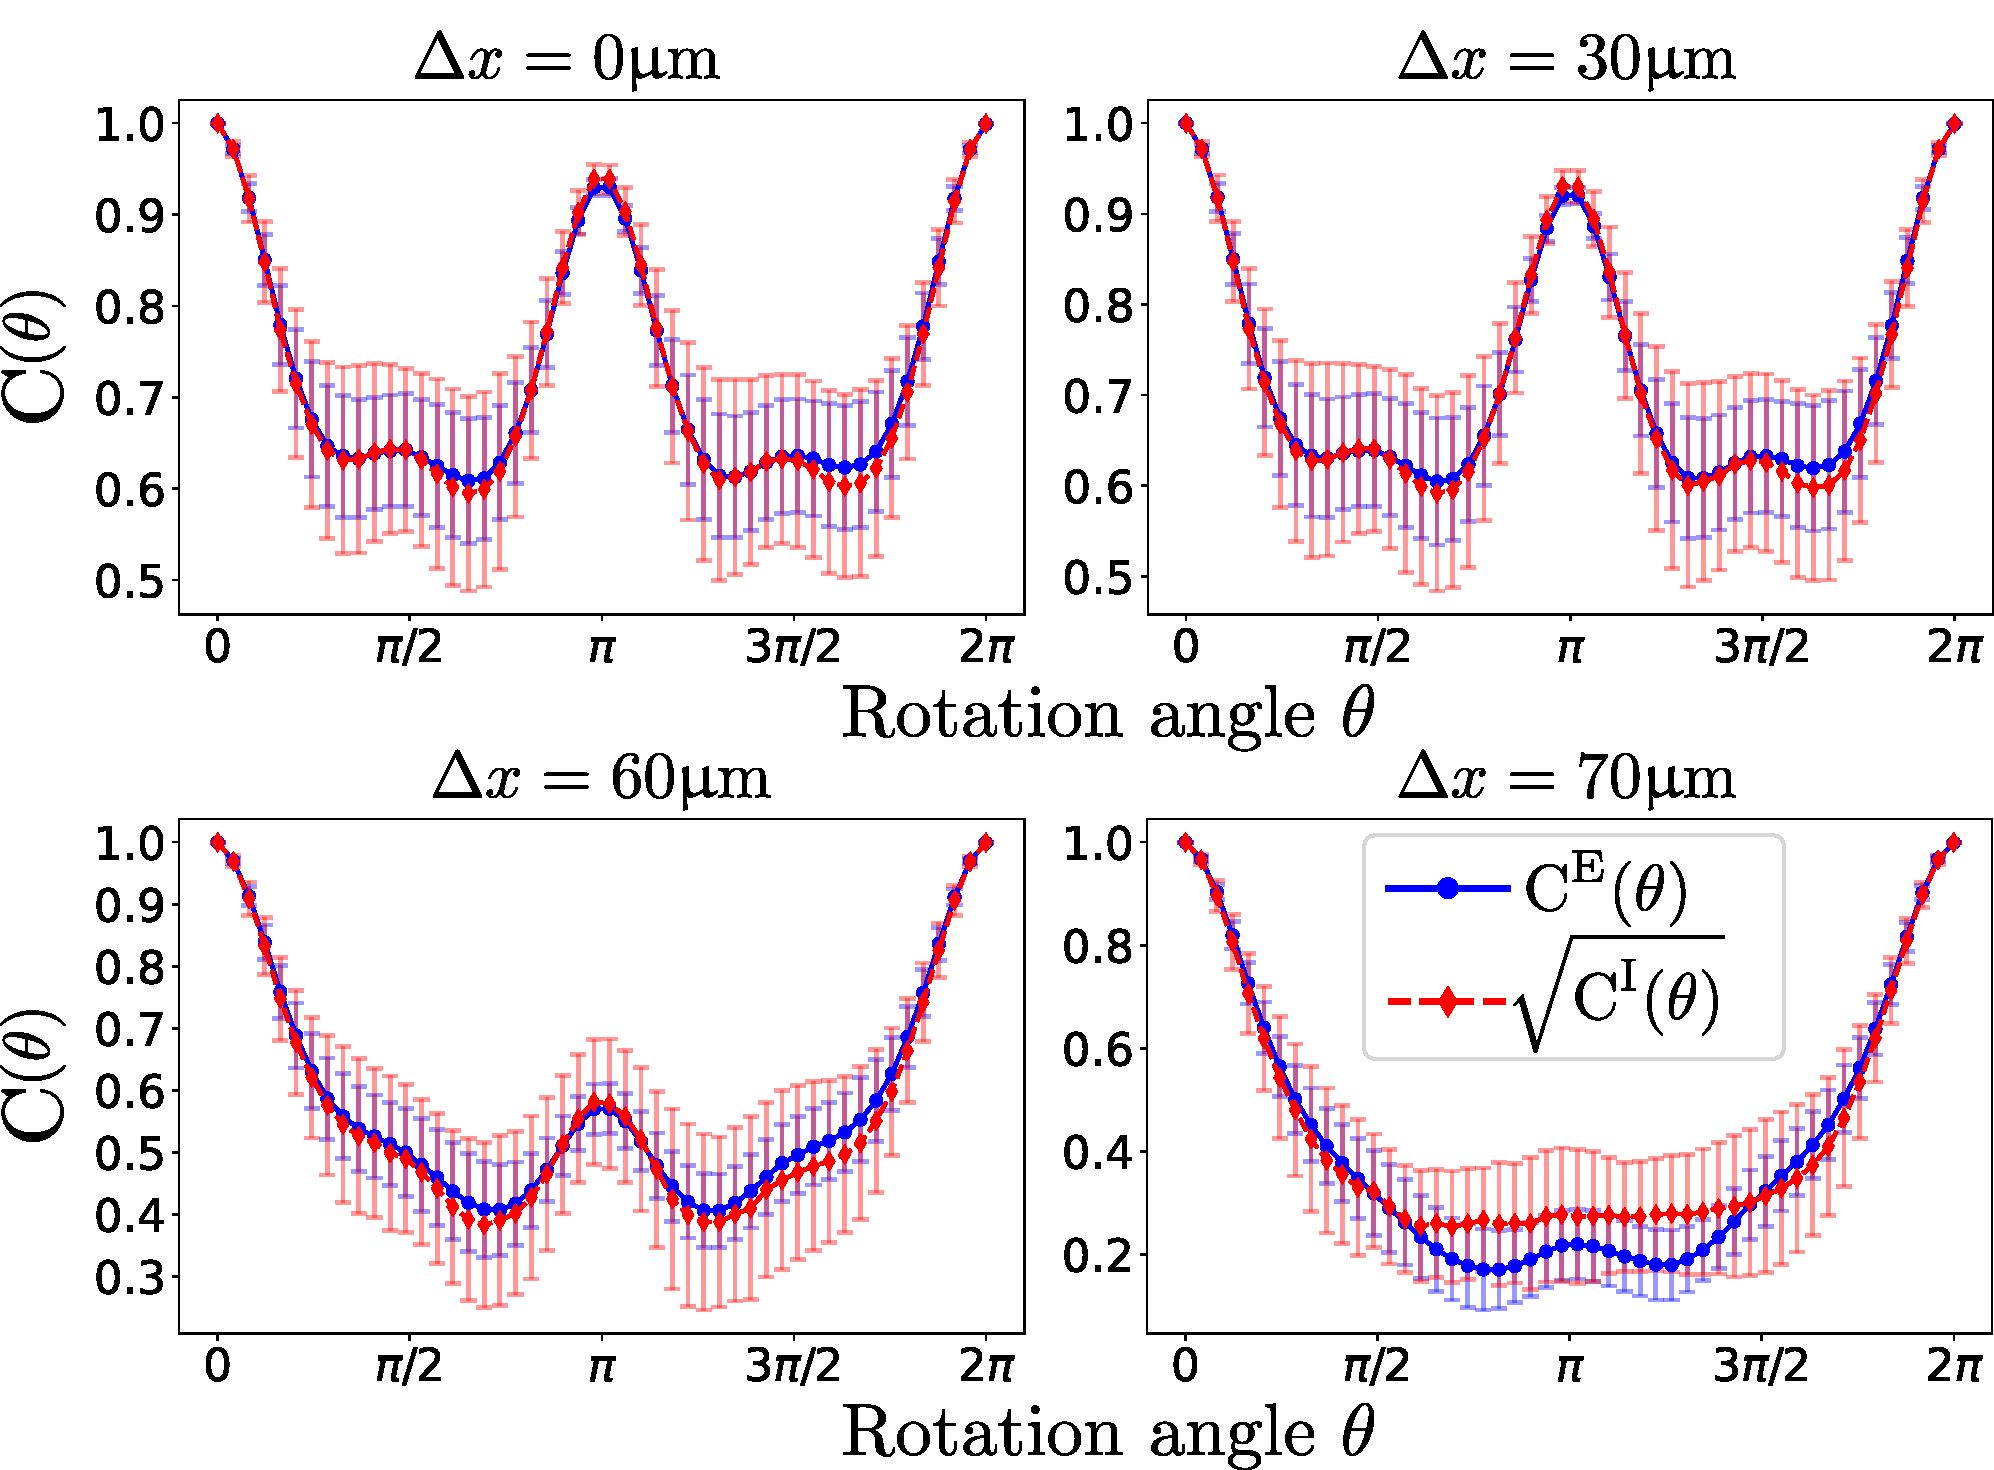
\includegraphics[width=0.90\textwidth]{images_si/FigSI_IvsE.pdf}
  \caption{\textbf{
  RME Correlation curves as a function of the rotation angle $\theta$ 
  computed from the field and the intensity ($\sqrt{C^I(\theta)}$) 
  for different values of the deformations.
  }
    Plain blue curves represents the estimation of the field correlation 
  directly from the field using Eq.~X of the main text ($C^E(\theta$) 
  and the dashed red curves represent the square root or the intensity correlation 
  computed using Eq.~\ref{Eq:CI}.
  $\Delta x$ represent the translation distance imposed to create the local deformation. 
  Error bars represent the standard deviation computed over 100 random input patterns. 
  
  }
\end{figure}
%   \includegraphics[width=0.85\textwidth]{SfigFullTMpixCpx_Dx0}
%   \caption{\textbf{Pixel basis TM.}
%   Complex amplitude of the elements of the pixel basis TM for both left and right circular polarizations 
%   in input and output 
%   for $\Delta x = 0$ \textmu m.
%   }



\section{Full mode basis transmission matrices before correction}



% \begin{figure}[H]
%   \centering
%   \includegraphics[width=0.60\textwidth]{SfigSVDs_Dx0}
%   \caption{\textbf{Singular values of the reference TM.}
%   Singular values of the pixel basis TM  (red), 
%   of the TM projected onto the mode basis before the correction of the aberrations (cyan),
%   and after the numerical optimization (blue) 
%   for $\Delta x = 0$ \textmu m.
%   The vertical dashed line indicates the theoretical number of modes (110).
%   Singular values are normalized by the maximal one in each case.
%   }
  
%     \centering
%   \includegraphics[width=0.60\textwidth]{SfigSVDs_Dx70}
%   \caption{\textbf{Singular values of the perturbed TM.}
%   Singular values of the pixel basis TM  (red), 
%   of the TM projected onto the mode basis before the correction of the aberrations (cyan),
%   and after the numerical optimization (blue)
%    for $\Delta x = 70$ \textmu m.
%   The vertical dashed line indicates the theoretical number of modes (110).
%   Singular values are normalized by the maximal one in each case.
%   }
% \end{figure}
% \clearpage





% \bibliographystyle{naturemag}

\bibliography{biblio}\newpage 

\end{document}

